\section{Zadanie projektowe}

Przy użyciu Algorytmu Ewolucyjnego zaprojektować sieć teleinformatyczną minimalizującą liczbę użytych systemów teletransmisyjnych o różnej modularności m (m = 1, m > 1 i m >> 1). Sieć opisana za pomocą grafu G = (N, E), gdzie N jest zbiorem węzłów, a E jest zbiorem krawędzi. Funkcja pojemności krawędzi opisana jest za pomocą wzoru, określonego w zadaniu. Zbiór zapotrzebowań D, pomiędzy każdą parą węzłów opisuje macierz zapotrzebowań i jest dany. Dla
każdego zapotrzebowania istnieją co najmniej 3 predefiniowane ścieżki. Sprawdzić,
jak wpływa na koszt rozwiązania agregacja zapotrzebowań, tzn. czy zapotrzebowanie realizowane jest na jednej ścieżce (pełna agregacja), czy dowolnie, na
wszystkich ścieżkach w ramach zapotrzebowania (pełna dezagregacja). Dobrać
optymalne prawdopodobieństwo operatorów genetycznych oraz liczność populacji. Dane pobrać ze strony http://sndlib.zib.de/home.action, dla sieci polska.

\section{Wyjaśnienie pojęć}
\label{section:explanation}

\subsection{Modularność}

Modularność określa maksymalną ilość zapotrzebowania, jaką można przepuścić przez krawędź, by zużyć jeden moduł (zwiększyć koszt o 1). Moduł zwiększa koszt niezależnie od stopnia wykorzystania, dlatego celem optymalizacji jest zminimalizowanie ich ilości poprzez odpowiedni dobór ścieżek dla zapotrzebowań.

Przykład: dla modularności = 30, jeśli dana krawędź ma obciążenie = 31, kosztuje ona 2 moduły. Jeśli dzięki optymalizacji obciążenie tej krawędzi zmalałoby do 30, kosztowałaby ona tylko 1 moduł.

\subsection{Algorytm Ewolucyjny}

Zgodnie z wykładami prof. Jarosława Arabasa, Algorytm Ewolucyjny opisuje się za pomocą algorytmu, ukazanego w rozdziale \ref{section:mainloop}. Na algorytm składają się następujące funkcjonalności:
\begin{enumerate}
    \item inicjalizacja populacji,
    \item główna pętla algorytmu ewolucyjnego,
    \item mutacja (ang. \textit{mutation}),
    \item krzyżowanie (ang. \textit{crossover}),
    \item selekcja (ang. \textit{selection}, oznaczane jako \textit{select}),
    \item warunek zatrzymania,
    \item funkcja celu.
\end{enumerate}

\section{Założenia projektu}

Projekt wykonywany jest w ramach przedmiotu Algorytmy Heurystyczne (ALHE) w semestrze zimowym 2020 na Wydziale EiTI Politechniki Warszawskiej. Prowadzącym projekt jest dr inż. Stanisław Kozdrowski.

Implementacja projektu jest wykonywana w języku Python. Algorytm ewolucyjny posiada własną implementację i nie jest zaczerpnięty z bibliotek zewnętrznych języka Python. Biblioteki narzędziowe języka Python, którymi się wspomagano, to między innymi biblioteki:
\begin{itemize}
    \item xml - do przeprowadzenia parsowania pliku XML do obiektów Python (rozdział \ref{section:preparing})
    \item tqdm - ukazywania paska postępu
    \item random - do generacji liczb pseudolosowych (użyto ziarna (ang. \textit{seed}))
    \item logging - do logowania informacji pomocniczych w czasie działania programu
    \item json - do zapisu i odczytu plików JSON.
\end{itemize}

W projekcie zaimplementowano możliwość uruchomienia programu dla sieci w pełni zagregowanej lub sieci w pełni rozproszonej (dezagregacja, ang. \textit{distributed}). Dodano także możliwość sterowania modularnością algorytmu.

\section{Przygotowanie danych}
\label{section:preparing}

Dla sieci ,,polska'', pobrano plik XML oraz TXT ze wszystkimi informacjami dla danych dotyczących terytorium Polski. Następnie, przeprowadzono analizę budowy plików oraz znaczenia poszczególnych terminów. Wyeliminowano z programu dane nieistotne dla rozwiązywanego problemu. Analiza znaczenia terminów przeprowadzona jest w rozdziale \ref{section:explanation}.

Następnie, zbudowano parser, konwertujący wybrane części pliku XML do obiektów języka Python. Budowa słowników i list, w których były przechowywane informacje o sieci, została przedstawiona na poniższym przykładzie:
\lstset{language=Python}
\begin{lstlisting}
nodes = ['Gdansk', 'Bydgoszcz', ...]

link_keys = [
    (0, 1),
    (0, 2),
    (1, 3),
]

links_array = [
    Link_0_1_data,
    Link_0_2_data,
    ...,
    Link_1_3_data,
    ...,
]

Link_a_b_data = {
    'setupCost': 156.0,
    'capacity0': 155.0,
    'capacity1': 622.0,
    'cost0': 156.0,
    'cost1': 468.0,
}

demand_array = [
    Demand_0_1_data,
    Demand_0_2_data,
    ...
]

Demand_a_b_data = {
    'demand': 195.00,
    'admissiblePaths': [
        [(0,2), (1,2)],
        [(0,10), (1,10)],
        [(0,2), (2,9), (7,9), (1,7)],
        ...
    ]
}

demand_keys = [
    (0, 1),
    (0, 2),
    (1, 2),
]

\end{lstlisting}

\section{Możliwość konfiguracji parametrów}

Zaimplementowano możliwość konfiguracji parametrów, dostępnych w czasie działania programu ze wszystkich plików programu, w słowniku \textit{settings}. W pliku \textit{config/config.txt} istnieje możliwość ustalenia własnych wartości parametrów, bez konieczności znajomości języka Python. Sposób definiowania parametrów to: <klucz>=<wartość>, np. MODULARITY=5.

W pliku \textit{config.txt}, prawda definiowana jest jako 1, fałsz jako 0. Później wartość parametru jest konwertowana na typ \textit{bool} w języku Python.

W języku Python zapisane są ustawienia domyślne, które są nadpisywane przez ustawienia pliku \textit{config.txt}. Można ustawić następujące parametry:
\begin{itemize}
    \item LAMBDA - liczba chromosomów w każdej kolejnej populacji,
    \item MI - liczba chromosomów w populacji początkowej,
    \item CROSSOVER\_PROB - prawdopodobieństwo krzyżowania,
    \item CROSSOVER\_POINTS\_COUNT - liczba punktów krzyżowania (domyślnie 2),
    \item MUTATION\_PROB - prawdopodobieństwo mutacji,
    \item TARGET\_FITNESS - docelowa wartość funkcji celu (jeden z warunków wystarczających zatrzymania),
    \item MAX\_GENERATIONS - maksymalna liczba pokoleń (jeden z warunków wystarczających zatrzymania),
    \item MAX\_STALE\_GENERATIONS - maksymalna liczba niepoprawiających się pokoleń (jeden z warunków wystarczających zatrzymania),
    \item DISTRIBUTED - określa czy algorytm jest rozproszony (1), albo zagregowany (0),
    \item MODULARITY - modularność algorytmu,
    \item TOURNAMENT\_COMPETITION\_COUNT - wielkość szranek selekcji turniejowej,
    \item SEED - wartość ziarna generacji liczb pseudolosowych (podczas testowania ustawiona na 74),
    \item SHOW\_LOG\_ON\_CONSOLE - czy propagować logi programu na konsolę użytkownika,
    \item MUTATION\_FREQUENCY - określa ilość genów zmutowanych w pojedynczym osobniku. Pojedynczy gen może zmutować wielokrotnie w trakcie jednej mutacji. Żaden gen nie zmutuje, jeśli nie powiedzie się test na prawdopodobieństwo mutacji.
\end{itemize}

\section{Charakterystyka implementacji algorytmu}

\subsection{Inicjalizacja populacji}

Standardowa procedura inicjalizacji losuje wartości chromosomów z całej przestrzeni przeszukiwań i zwraca uzyskaną populację.

\subsection{Główna pętla algorytmu}
\label{section:mainloop}

Zgodnie z działaniem algorytmu ewolucyjnego, główna pętla algorytmu, umieszczona w pliku \textit{src/main.py}, wywołuje funkcje z pozostałych plików programu i steruje przebiegiem pętli. Algorytm pętli głównej został ukazany poniżej:
\lstset{language=Python}
\begin{lstlisting}
createInitPopulation(MI)
t = 0
while not stop_condition(t, stale_generations_count, lowest_fitness):
    pop = []
    for i in range(settings["LAMBDA"]):
        a = random.uniform(0, 1)
        if a < settings["CROSSOVER_PROB"]:
            chromosome = mutation(crossover(select(populations[t], k=2)))
            pop += chromosome
        else:
            chromosome = mutation(select(populations[t], k=1))
            pop += chromosome
    populations += pop
    t += 1
\end{lstlisting}

\subsection{Mutacja}

Jeżeli wartość parametru MUTATION\_FREQUENCY jest równa -1, wtedy mutacja wykonywana jest na jednym, wybranym losowo z rozkładem jednostajnym, genie z populacji. Jeżeli wartość tego parametru jest w granicach od 0 do 1, taki procent liczby genów zostaje wylosowany ze zwracaniem z populacji i poddany mutacji. Mutacja polega na zmianie wylosowanego genu na wartość, wylosowaną ze wszystkich dostępnych wartości.

\subsection{Krzyżowanie}

Krzyżowanie jest wielopunktowe, zawsze z dwóch osobników powstaje jeden skrzyżowany. Liczbę punktów krzyżowania określa się w parametrze CROSSOVER\_POINTS\_COUNT, domyślnie równym 2.

\subsection{Selekcja}

Selekcja jest turniejowa. Z rozkładem jednostajnym bez zwracania losowane są różne chromosomy do szranek. Wielkość szranek jest określona w parametrze TOURNAMENT\_COMPETITION\_COUNT, domyślnie równym 2.

\subsection{Warunek zatrzymania}

Algorytm zatrzymuje się, jeżeli wydarzy się co najmniej jedno z trzech zdarzeń:
\begin{itemize}
    \item osiągnięta została maksymalna liczba pokoleń (MAX\_GENERATIONS)
    \item osiągnięta została maksymalna liczba niepolepszających pokoleń (MAX\_STALE\_GENERATIONS)
    \item osiągnięta została pożądana wartość funkcji celu (TARGET\_FITNESS)
\end{itemize}

\subsection{Funkcja celu}

Jest obliczana zgodnie z zasadami, opisanymi w zadaniu. Chromosom zagregowany składa się z liczb od 0 do 5, oznaczających indeksy dozwolonych ścieżek dla kolejnych zapotrzebowań. Chromosom rozproszony zaś, składa się z liczb od 0 do 1 dla każdej dozwolonej ścieżki dla kolejnych zapotrzebowań. Później finalna wartość procentowa przepływu daną dozwoloną ścieżką jest wartością znormalizowaną w ramach każdego zapotrzebowania.

\section{Analiza wyników}

Przykłady wartości funkcji celu w zależności od pokolenia są ukazane na rysunkach \ref{fig:a} oraz \ref{fig:b}.

\begin{figure}[h!]
    \centering
    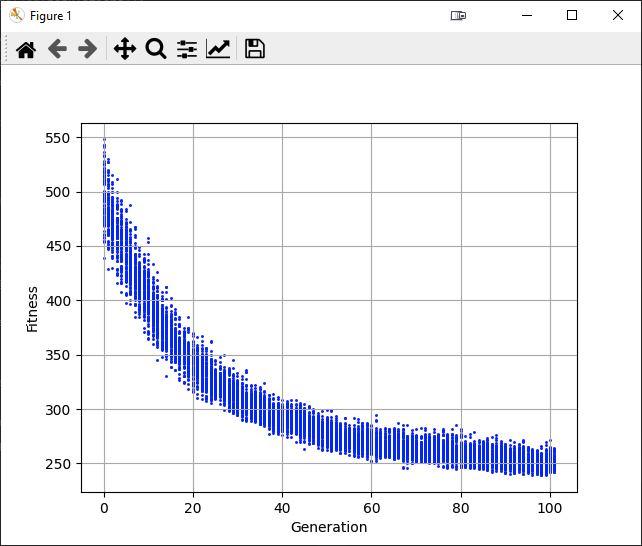
\includegraphics[width=\textwidth]{img/wykres.png}
    \caption{Wartość funkcji celu w zależności od populacji. Wykres 1}
    \label{fig:a}
\end{figure}

\begin{figure}[h!]
    \centering
    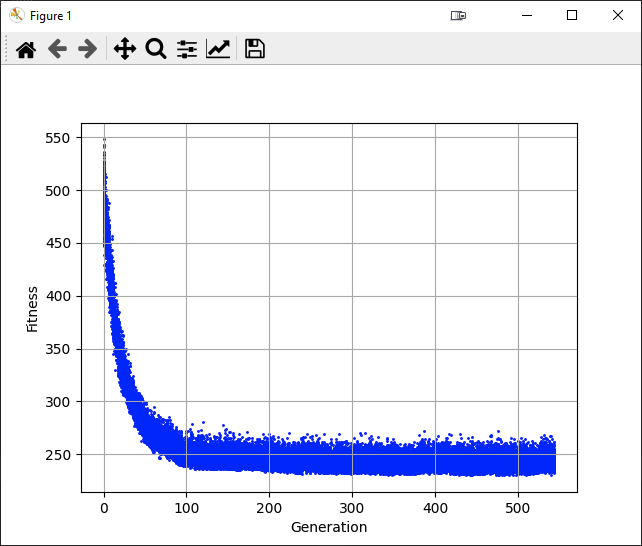
\includegraphics[width=\textwidth]{img/wykres2.png}
    \caption{Wartość funkcji celu w zależności od populacji. Wykres 2}
    \label{fig:b}
\end{figure}

Zgodnie z tabelą \ref{table:results}, przeprowadzono testy, aby sprawdzić dla różnych modularności  i agregacji lub rozproszenia, jak zależą wartości parametrów algorytmu od prezentowanych wyników. 

Przy agregacji dla modularności = 1 znaczenie ma tylko długość ścieżek, z uwagi na fakt, że zapotrzebowania są zawsze liczbami całkowitymi, dla zapotrzebowania D potrzebne jest D * długość ścieżki modułów. Przyglądając się wynikom można podejrzewać, że 22444 to minimum globalne danego problemu. Dwóm przejściom algorytmu nie udało się osiągnąć tego wyniku, najprawdopodobniej w wyniku niesprzyjających mutacji lub zbyt małej ilości generacji.

Modularność 5 pozwala już na delikatne optymalizacje/straty w wyniku w zależności od wykorzystania ostatniego z modułów na każdej krawędzi. Osiągany wynik 4494 różni się o raptem 5, jeśli porównać go z wynikiem modularności = 1 (22444 / 5 = 4488,8), więc zakładając, że algorytm dla modularności = 1 osiągnął minimum globalne, to wynik ten można by poprawić jedynie o 5, czyli 0,1\%.

Dla modularności = 100 przewidywany najlepszy wynik to 225 (zgodnie z logiką z poprzednich rozważań). Algorytm osiągnął zbliżony wynik w prawie każdym przypadku. 

Analiza wyników algorytmu w wersji zagregowanej pozwala stwierdzić, że wybrane parametry pozwalają osiągnąć zadowalające wyniki. Prawdopodobnie algorytmy osiągają swoje docelowe wartości dość szybko, a następnie pracują do momentu osiągnięcia założonej ilości generacji. W takiej sytuacji dalszych optymalizacji można by poszukiwać w skróceniu ilości generacji, a zaoszczędzony czas przeznaczyć na wielokrotne uruchomienia lub na zwiększenie populacji, lub też poprzez zwiększenie ilości mutujących genów w osobniku, by osiągnąć większą eksplorację.

Algorytm w wersji rozproszonej wykonuje się znacznie dłużej z uwagi na znacznie zwiększoną ilość operacji. Pomimo tego, dla modularności = 1 osiąga on gorsze wyniki od wersji zagregowanej. Wynika to z faktu, iż teraz na ścieżce umieszczana jest tylko część zapotrzebowania, która najprawdopodobniej posiada część ułamkową. Takie pozostałości wymagają wykorzystania większej ilości modułów, jednocześnie nie oferując żadnego zysku. Algorytm rozproszony ma szansę stać się skuteczniejszy od zagregowanego w sytuacji, kiedy modularność osiągnie na tyle duże wartości, że będzie się opłacało przepuścić część zapotrzebowania dłuższą ścieżką, aby dopełnić niewykorzystane w pełni moduły.

\begin{table}[h!]
    \centering
    \begin{tabular}{||c c c c||} 
     \hline
     Mi,Lambda,Mut,Cross,Stale & Rozproszony & Modularność & Wynik \\ [0.5ex] 
     \hline\hline
     1000;1000;0,7;0,9;500 & Agregacja & 1 & 34624.0 \\
     1000;1000;0,7;0,9;500 & Agregacja & 1 & 22444,00 \\
     1000;1000;0,5;0,9;500 & Agregacja & 1 & 22444,00 \\
     1000;1000;0,95;0,95;500 & Agregacja & 1 & 22444,00 \\
     2000;2000;0,95;0,95;400 & Agregacja & 1 & 22444,00 \\
     20000;1500;0,95;0,95;300 & Agregacja & 1 & 22444,00 \\
     600;300;0,95;0,5;300 & Agregacja & 1 & 23438,00 \\
     600;300;0,95;0,95;600 & Agregacja & 1 & 22444,00 \\
     \hline
     600;300;0,95;0,95;600 & Agregacja & 5 & 4494,00 \\
     600;300;0,95;0,95;600 & Agregacja & 5 & 4494,00 \\
     700;500;1;1;600 & Agregacja & 5 & 4493,00 \\
     \hline
     700;500;1;1;600 & Agregacja & 100 & 231,00 \\
     700;500;1;0,8;600 & Agregacja & 100 & 231,00 \\
     50;100;1;1;600 & Agregacja & 100 & 230,00 \\
     50;100;1;0,5;600 & Agregacja & 100 & 245,00 \\
     50;100;0,5;1;600 & Agregacja & 100 & 230,00 \\
     50;100;0,5;0,8;600 & Agregacja & 100 & 230,00 \\
     \hline
     50;100;0,5;0,8;600 & Rozproszony & 1 & 24012,00 \\
     1000;100;0,5;0,8;30 & Rozproszony & 1 & 25934,00 \\
     1000;200;0,5;0,8;30 & Rozproszony & 1 & 24862.00 \\
     50;40;0,5;0,8;30 & Rozproszony & 1 & 29184,00 \\
     50;40;1;1;150 & Rozproszony & 1 & 28993,00 \\
     \hline
     50;100;0,9;0,9;80 & Rozproszony & 5 & 5410,00 \\
     1000;200;0,9;0,9;30 & Rozproszony & 5 & 5394,00 \\
     \hline
     1000;200;0,9;0,9;30 & Rozproszony & 100 & 313,00 \\
     50;100;0,9;0,9;60 & Rozproszony & 100 & 332,00 \\
     200;50;0,9;0,9;250 & Rozproszony & 100 & 318,00 \\   
     \hline
    \end{tabular}
    \caption{Wyniki testów.}
    \label{table:results}
\end{table}